\documentclass[screen, aspectratio=169]{beamer}
\usepackage[T1]{fontenc}
\usepackage[utf8]{inputenc}
\usepackage{tikz, environ, siunitx, pgfpages, xcolor}
\usepackage{listings}

\usetikzlibrary{shapes.geometric,arrows, positioning, calc}

%\setbeameroption{show notes on second screen=right}

% Use the NTNU-temaet for beamer 
% \usetheme[style=ntnu|simple|vertical|horizontal, 
%     language=bm|nn|en, 
%     smalltitle, 
%     city=all|trondheim|alesund|gjovik]{ntnu2017}
\usetheme[style=horizontal,language=bm]{ntnu2015}

\usepackage[norsk]{babel}

\title[Short title]{Øvingsforelesning 2 Python (TDT4110)}
\subtitle{Introduksjon, Kalkulasjoner}
\author[O.M. Pedersen]{Ole-Magnus Pedersen}
\institute[NTNU]{}
\date{}
%\date{} % To have an empty date

\NewEnviron{transparent}{
	\tikz\node[opacity=0.2,align=left,inner xsep=0]{\parbox[t]{\linewidth}{
			\BODY
		}};
	}

\lstset{language=Python}
\RequirePackage{listings, color, textcomp}
\lstset{
	tabsize=2,
	rulecolor=,
	basicstyle=\ttfamily\small,
	upquote=true,
	aboveskip={1.5\baselineskip},
	columns=fixed,
	showstringspaces=false,
	extendedchars=true,
	literate={æ}{{\ae}}1
			 {ø}{{{\o}}}1
			 {å}{{\aa}}1
			 {Æ}{{\AE}}1
			 {Ø}{{\O}}1
			 {Å}{{\AA}}1,
	breaklines=true,
	breakatwhitespace=true,
	escapeinside={(*}{*)},
	showtabs=false,
	showspaces=false,
	keepspaces=true,
	showstringspaces=false,
	frame=l,
	identifierstyle=\ttfamily,
	keywordstyle=\color[rgb]{1.0,0,0},
	keywordstyle=[1]\color[rgb]{0,0,0.75},
	%keywordstyle=[2]\color[rgb]{0.5,0.0,0.0},
	keywordstyle=[3]\color[rgb]{0.127,0.427,0.514},
	keywordstyle=[4]\color[rgb]{0.4,0.4,0.4},
	commentstyle=\color[rgb]{0.133,0.545,0.133},
	stringstyle=\color[rgb]{0.639,0.082,0.082},
	mathescape
}

\definecolor{secondaryColor}{RGB}{121, 162, 206}

\tikzstyle{process} = [rectangle, minimum width=2cm, minimum height=1cm, text centered, draw=black, fill=secondaryColor]
\tikzstyle{decision} = [diamond, minimum width=2cm, minimum height=1cm, text centered, draw=black, fill=secondaryColor]

\hypersetup{
	colorlinks,
	urlcolor={blue!70!black}
}

\begin{document}

\begin{frame}
  \titlepage
\end{frame}

% Alternatively, special title page command to get a different background
% \ntnutitlepage

\begin{frame}{Oversikt}
	\begin{itemize}
			\item Praktisk Info
			\begin{transparent}
				\item Repetisjon fra sist
				\item Oppgaver for øving 2
			\end{transparent}
	\end{itemize}
\end{frame}

\begin{frame}{Praktisk Info}
	\begin{itemize}
		\item Last opp øvinger på Blackboard før godkjenning
		\item Bruk studasser
		%\item<+-> QueueMe
	\end{itemize}
\end{frame}

%{ % all template changes are local to this group.
%	\setbeamertemplate{navigation symbols}{}
%	\begin{frame}[plain]
%		\begin{tikzpicture}[remember picture,overlay]
%		\node[at=(current page.center)] {
%			
\includegraphics[page=1, width=\paperwidth]{QueueMePresentasjonPP.pdf}
%		};
%		\end{tikzpicture}
%	\end{frame}
%	\begin{frame}[plain]
%		\begin{tikzpicture}[remember picture,overlay]
%		\node[at=(current page.center)] {
%			
\includegraphics[page=2, width=\paperwidth]{QueueMePresentasjonPP.pdf}
%		};
%		\end{tikzpicture}
%	\end{frame}
%	\begin{frame}[plain]
%		\begin{tikzpicture}[remember picture,overlay]
%		\node[at=(current page.center)] {
%			
\includegraphics[page=3, width=\paperwidth]{QueueMePresentasjonPP.pdf}
%		};
%		\end{tikzpicture}
%	\end{frame}
%}

\begin{frame}{Oversikt}
	\begin{itemize}
		\begin{transparent}
			\item Praktisk Info
		\end{transparent}
		\item Repetisjon fra sist
		\begin{transparent}
			\item Oppgaver for øving 2
		\end{transparent}
	\end{itemize}
\end{frame}

\begin{frame}[fragile]{Matte}
	\begin{columns}
		\begin{column}{.5\textwidth}
			\begin{itemize}
				\item \lstinline|+, -, *, /|
				\item \lstinline|>, <, ==, %, //, **|
				\vspace{2em}
				\item<2-> Oppgave: Skriv et program som regner ut resten når $2^7$ deles på $42$.
			\end{itemize}
		\end{column}
		\begin{column}{.4\textwidth}
			\footnotesize
			\begin{block}{\small Presedens og parantesbruk}
				\begin{enumerate}
					\item \lstinline|-| \hfill negasjon
					\item \lstinline|* / // %| \hfill multiplikasjon, divisjon, \\\hfill heltallsdivisjon, modulo
					\item \lstinline|+ -| \hfill addisjon, subtraksjon
				\end{enumerate}
				\begin{itemize}
					\item Fra venstre mot høyre
					\item Innenfra og ut
				\end{itemize}
			\end{block}
		\end{column}
	\end{columns}
\end{frame}

\begin{frame}[fragile]{Variabler}
	\begin{itemize}
		\item Navngitte plasseringer i minne hvor man kan lagre verdier
		\begin{description}
			\item[Integer] Heltallsverdi
			\item[Float] Desimaltall
			\item[Boolean] Kan ha nøyaktig to verdier, \lstinline|True| og \lstinline|False|
			\item[String] Tekst
		\end{description}
		\item Vær nøye med hva slags typer variablene dine har
		\begin{itemize}
			\item \lstinline|input()| gir en string
		\end{itemize}
	\end{itemize}
\end{frame}

\begin{frame}[fragile]{Innebygde funksjoner}
	\begin{itemize}
		\item \lstinline|round()|
		\item \lstinline|abs()|
		\item \lstinline|min()|
		\item \lstinline|input()|
		\item \lstinline|print()|
	\end{itemize}
\end{frame}

\begin{frame}{Oppgave}
	\begin{itemize}
		\item Skriv et program som spør om et desimaltall, lagrer det i en variabel, beregner absoluttverdien og skriver ut ''|<tall1>| = <absoluttverdi av tall1>''
	\end{itemize}
\end{frame}

\begin{frame}{Importere moduler}
	\begin{itemize}
		\item Inneholder kode for å gjøre ting uten å måtte skrive egne funksjoner for det:
		\begin{itemize}
			\item Matte
			\item Grafiske brukergrensesnitt
			\item Lese spesielle filtyper
		\end{itemize}
		\item \lstinline|import math|
		\item \lstinline|from math import pi|
	\end{itemize}
\end{frame}

\begin{frame}[fragile]{Oppgave}
	\begin{itemize}
		\item Lag et program som ber om radius og høyde til en sylinder, regner ut volumet og skriver det ut til 5 desimalers nøyaktighet
		\begin{itemize}
			\item $V=\pi r^2 h$
			\item \lstinline|import math|, \lstinline|math.pi|, \lstinline|round(tall, desimaler)|
		\end{itemize}
	\end{itemize}
\end{frame}

\begin{frame}{Oversikt}
	\begin{itemize}
		\begin{transparent}
			\item Praktisk Info
			\item Repetisjon fra sist
		\end{transparent}
			\item Oppgaver for øving 2
	\end{itemize}
\end{frame}

\begin{frame}[fragile]{Logikk}
	\only<-5>{
		\begin{itemize}
			\item Boolske uttrykk
			\begin{itemize}
				\item Har verdi \lstinline|True| eller \lstinline|False|
			\end{itemize}
			\item Uttrykk består av:
			\begin{itemize}
				\item<2-> Boolske (boolean) variabler
				\item<3-> \lstinline|and, or, not|
				\item<4-> Sammenligninger med \lstinline|==, !=, >, >=, <, <=, is, is not|
			\end{itemize}
			\item<5-> Eksempler (\lstinline|a = False, b = True| er boolske, \lstinline|x = 23, y = 25| er integers):
			\begin{itemize}
				\item<5> \lstinline|b|
				\item<5> \lstinline|b and not a|
				\item<5> \lstinline|x == 2 + y|
				\item<5> \lstinline|not ((a and b) or x != y)|
			\end{itemize}	
		\end{itemize}
	}
	\only<6>{
		\begin{itemize}
			\item Boolske uttrykk
			\begin{itemize}
				\item Har verdi \lstinline|True| eller \lstinline|False|
			\end{itemize}
			\item Uttrykk består av:
			\begin{itemize}
				\item<2-> Boolske (boolean) variabler
				\item<3-> \lstinline|and, or, not|
				\item<4-> Sammenligninger med \lstinline|==, !=, >, >=, <, <=, is, is not|
			\end{itemize}
			\item<5-> Eksempler (\lstinline|a = False, b = True| er boolske, \lstinline|x = 23, y = 25| er integers):
			\begin{itemize}
				\item \lstinline|b --> True|
				\item \lstinline|b and not a --> True|
				\item \lstinline|x == 2 + y --> False|
				\item \lstinline|not ((a and b) or x != y) --> False|
			\end{itemize}	
		\end{itemize}
		}
\end{frame}

\begin{frame}{Oppgave}
	\begin{itemize}
		\item Skriv et program som spør en bruker om tre tall og sjekker om summen av de to første er lik det tredje
	\end{itemize}
\end{frame}

\begin{frame}{Oppgave}
	\begin{itemize}
		\item Skriv et program som tar inn et tall og sjekker om det er et partall
		\begin{itemize}
			\item<2-> Hint: Sjekk om resten er 0 når det deles på to
		\end{itemize}
	\end{itemize}
\end{frame}

\begin{frame}{Oppgave}
	\begin{itemize}
		\item Lag et program som ber om et passord og sjekker om det er likt et passord du har lagret som en variabel.
	\end{itemize}
\end{frame}

\begin{frame}[fragile]{if-setninger}
	\begin{columns}
		\begin{column}{.4\textwidth}
			\begin{itemize}
				\item Kjør koden inne i if-setningen dersom en betingelse er oppfylt
				\begin{itemize}
					\item Betingelse må være et logisk uttrykk
				\end{itemize}
				\item Kan nestes (en \lstinline|if| i en \lstinline|if| i en \lstinline|if| ...)
			\end{itemize}
			\begin{onlyenv}<1>
			\begin{lstlisting}
if <condition>:
	code to run
			\end{lstlisting}
			\end{onlyenv}
			\begin{onlyenv}<2->
				\begin{lstlisting}
if x > 10:
	print("Du vinner!")
				\end{lstlisting}
				\end{onlyenv}
		\end{column}
		\begin{column}{.6\textwidth}
			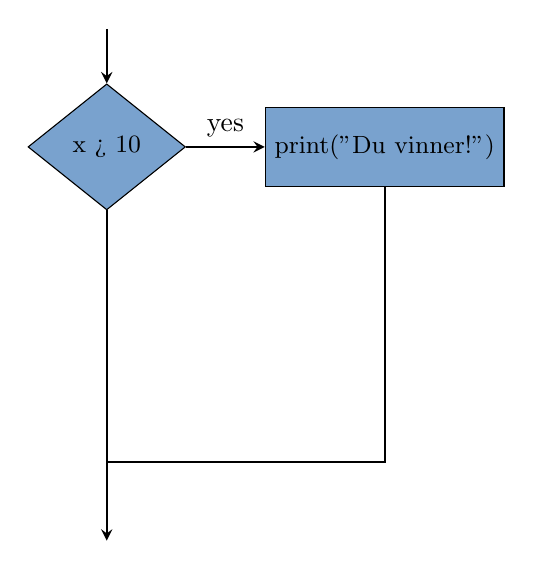
\begin{tikzpicture}[node distance=1cm and 1cm]
				\node (dec) [decision]{\small x > 10};
				\node (win) [process, right=of dec]{\small print(''Du vinner!'')};
				
				\draw[thick,->,>=stealth] (0,1.5) -- (dec);
				\draw[thick,->,>=stealth] (dec) -- node[anchor=south] {yes} (win);
				\draw[thick,->,>=stealth] (dec) -- (0, -5);
				\draw[thick] (win) -- ($ (win) + (0, -4) $) -- (0, -4);
			\end{tikzpicture}
		\end{column}
	\end{columns}
\end{frame}

\begin{frame}{Oppgave}
	\begin{itemize}
		\item Lag et program som tar inn et tall og skriver ut ''<tall> er et partall'' hvis det er et partall.
	\end{itemize}
\end{frame}

\begin{frame}{Oppgave}
	\begin{itemize}
		\item Lag et program som spør om et etternavn. Hvis det er likt ditt etternavn skal det skrive ut ''Dette er en match!!'' 
	\end{itemize}
\end{frame}

\begin{frame}[fragile]{Else}
	\begin{columns}
		\begin{column}{.4\textwidth}
			\begin{itemize}
				\item Koden i else-blokken kjøres dersom betingelsen ikke er sann
			\end{itemize}
			\begin{onlyenv}<1>
				\begin{lstlisting}
if <condition>:
	code to run if true
else:
	code to run if false
				\end{lstlisting}
			\end{onlyenv}
			\begin{onlyenv}<2->
				\begin{lstlisting}
if x > 10:
	print("Du vinner!")
else:
	print("Du taper!")
				\end{lstlisting}
			\end{onlyenv}
		\end{column}
		\begin{column}{.6\textwidth}
			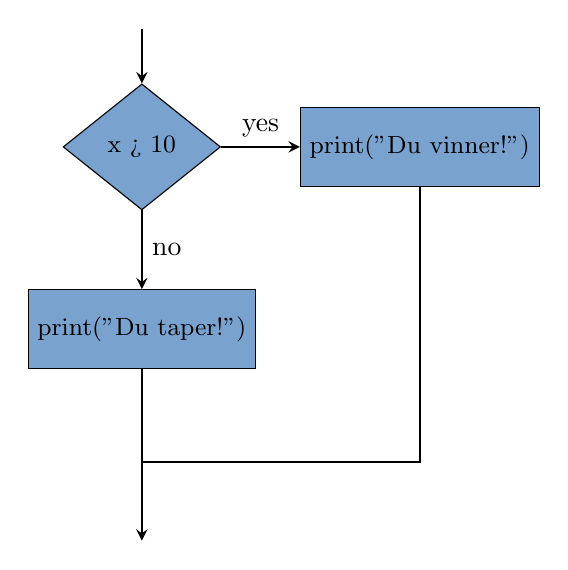
\begin{tikzpicture}[node distance=1cm and 1cm]
			\node (dec) [decision]{\small x > 10};
			\node (win) [process, right=of dec]{\small print(''Du vinner!'')};
			\node (lose) [process, below=of dec]{\small print(''Du taper!'')};
			
			\draw[thick,->,>=stealth] (0,1.5) -- (dec);
			\draw[thick,->,>=stealth] (dec) -- node[anchor=south] {yes} (win);
			\draw[thick,->,>=stealth] (dec) -- node[anchor=west] {no} (lose);
			\draw[thick,->,>=stealth] (lose) -- (0,-5);
			\draw[thick] (win) -- ($ (win) + (0, -4) $) -- (0, -4);
			\end{tikzpicture}
		\end{column}
	\end{columns}
\end{frame}

\begin{frame}{Oppgave}
	\begin{itemize}
		\item Lag et program som tar inn to tall. Programmet skal skrive ut ''<tall1> er større enn eller lik <tall2>'' eller ''<tall1> er mindre enn <tall2>'' avhengig av tallene.
		\item<2> Utvid programmet til å gi en spesiell beskjed dersom tallene er like
	\end{itemize}
\end{frame}

\begin{frame}{Oppgave}
	\begin{itemize}
		\item Kjell trenger help til å bestemme hva han skal ha med til lunsj. Han har en regel han vil følge, men sliter med å huske den. Regelen er:
		\begin{itemize}
			\item På mandag, onsdag og fredag spiser han brødskive med geitost
			\item På tirsdag og torsdag spiser han rundstykke med salami.
		\end{itemize}
		\item Lag et program der Kjell kan skrive inn hvilken ukedag det er, og får vite hva han skal ha til lunsj.
	\end{itemize}
\end{frame}

\begin{frame}[fragile]{Elif}
	\begin{columns}
		\begin{column}{.5\textwidth}
			\begin{itemize}
				\item Når du har flere muligheter for hva som kan skje
				\item \lstinline|elif|-koden kjøres bare dersom \lstinline|if|-betingelsen er \lstinline|False|
				\item Flere \lstinline|elif| kan settes opp etter hverandre
			\end{itemize}
			\vspace{-1em}
			\begin{onlyenv}<1>
				\begin{lstlisting}
if <condition1>:
	code if condition1 is True
elif <condition2>:
	code if condition1 is False and condition2 is True
else:
	code if no condition is True
				\end{lstlisting}
			\end{onlyenv}
			\begin{onlyenv}<2->
				\begin{lstlisting}
if x > 10:
	print("Vinn!")
elif x > 5:
	print("OK!")
else:
	print("Taper!")
				\end{lstlisting}
			\end{onlyenv}
		\end{column}
		\begin{column}{.5\textwidth}
			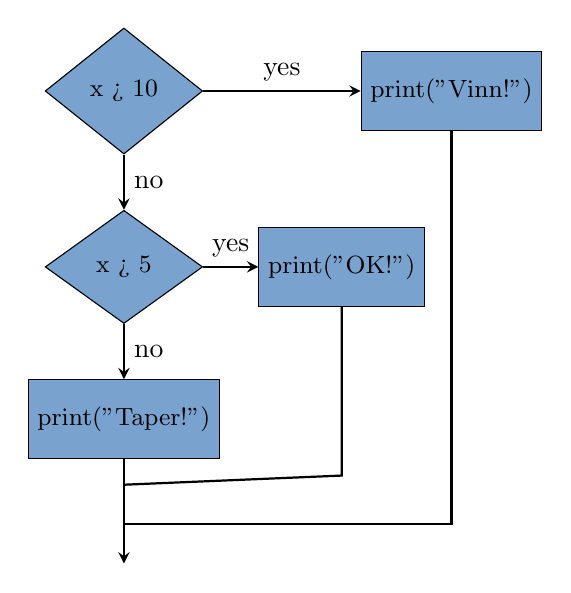
\begin{tikzpicture}[node distance=.7cm]
			\node (dec1) [decision]{\small x > 10};
			\node (win) [process, right=2cm of dec1]{\small print(''Vinn!'')};
			\node (dec2) [decision, below= of dec1]{\small x > 5};
			\node (mid) [process, right= of dec2]{\small print(''OK!'')};
			\node (lose) [process, below= of dec2]{\small print(''Taper!'')};
			
			\draw[thick,->,>=stealth] (dec1) -- node[anchor=south]{yes} (win);
			\draw[thick,->,>=stealth] (dec1) -- node[anchor=west]{no} (dec2);
			\draw[thick] (win) -- ($(win) + (0, -5.5)$) -- (0, -5.5);
			
			\draw[thick,->,>=stealth] (dec2) -- node[anchor=south]{yes} (mid);
			\draw[thick,->,>=stealth] (dec2) -- node[anchor=west]{no} (lose);
			\draw[thick] (mid) -- ($(mid) + (0, -2.65)$) -- (0, -5);
			
			\draw[thick,->,>=stealth] (lose) -- (0, -6);
			\end{tikzpicture}
		\end{column}
	\end{columns}
\end{frame}

\begin{frame}{Oppgave}
	\begin{itemize}
		\item Lage et program som tar inn to tall (kalt tall1 og tall2). 
		\begin{itemize}
			\item Dersom de er like skal programmet skrive ut ''Gratulerer, tallene er like''
			\item Hvis tall1 er større enn tall2 skal det skrive ut ''Tall1 er <differanse mellom tallene> større enn tall2''.
			\item Dersom tall2 er større enn tall1 skal programmet skrive ut ''Tall1 er <differanse mellom tallene> mindre enn tall2''.
		\end{itemize}
		\item Til slutt skal programmet skrive ut ''Takk for denne gang''
	\end{itemize}
\end{frame}

\begin{frame}{Oppgave}
	\begin{itemize}
		\item Lag et program som tar inn et heltall (kalt $x$ her) fra brukeren. Avhengig av tallet skal følgende skje:
		\begin{itemize}
			\item Dersom $x$ er et primtall mindre enn 30 (altså et av 2, 3, 5, 7, 11, 13, 17, 19, 23, 29) skal programmet si ifra om dette
			\item Ellers, dersom $x$ er delelig på 4 skal programmet si hva $\frac{x}{4}$ er
			\item Ellers, dersom $x$ er odde skal programmet si ifra om dette
			\item Ellers skal programmet si hva $\frac{x}{2}$ er.
		\end{itemize}
	\end{itemize}
\end{frame}

\begin{frame}[fragile]{Oppgave}
	\begin{itemize}
		\item Lag et program som tar inn en tekststreng fra brukeren. Ut i fra strengen skal følgende skje:
		\begin{itemize}
			\item Dersom strenger er lik ''IalwaysCheat'' skal programmet skrive ut ''Juksing er ikke lov, prøv igjen senere''
			\item Ellers, dersom lengden på strengen er større enn 4 og mindre enn 10 skal programmet skrive ut ''Dette var en streng med perfekt lengde''.
			\begin{itemize}
				\item \lstinline|len(streng)| gir lengden på strengen med navn ''streng''.
			\end{itemize}
			\item Ellers, hvis strengen starter på ''hei'' og har mer enn 6 tegn skal programmet skrive ut ''Hei på deg også''
			\begin{itemize}
				\item Hint: \lstinline|streng.startswith("hei")| gir \lstinline|True| hvis strengen starter med ''hei''
			\end{itemize}
			\item Ellers skal programmet skrive ut ''Dette var en kjedelig streng''
		\end{itemize}
	\end{itemize}
\end{frame}

\begin{frame}{Spørsmål}
	\begin{itemize}
		\item Spørsmål/kommentarer kan også sendes til \href{mailto:olemagnp@stud.ntnu.no}{olemagnp@stud.ntnu.no}
	\end{itemize}
\end{frame}

\end{document}